%форматирование размера документа
\documentclass[11pt, a4paper]{article}

\usepackage{geometry}
% total - determines printable width, height
\geometry{ 
	a4paper, total={160mm,267mm}
}

%----text,fonts------------------------------------------------------------------------------------
\usepackage{mmap}
\usepackage[T2A]{fontenc}
\usepackage[utf8]{inputenc}
\usepackage[english, russian]{babel}
\usepackage{setspace}
\setstretch{0,9}
\usepackage{fancyvrb}

%----math,graphics---------------------------------------------------------------------------------
\usepackage{amsmath,amsfonts,amssymb}
\usepackage{amsthm}
\usepackage{listings}

\usepackage{tikz}
\usetikzlibrary{calc}
\usepackage{pgfplots}
\pgfplotsset{
	compat=1.17
}

\usepackage{graphicx}
\graphicspath{{image/}}

\usepackage{wrapfig}
\usepackage{tabularx}

% relative importing
\usepackage{import}


\begin{document}

\import{.}{titular.tex}
\newpage

\section{Описание метода. Расчетные формулы}

Кубический сплайн - функция порядка 3. С помощью них можно строить функцию, которая бы проходила
через заданные точки, причем также на нее накладываются дополнительные ограничение: непрерывность
первой и второй производных.

\begin{figure}[h]
  \centering
  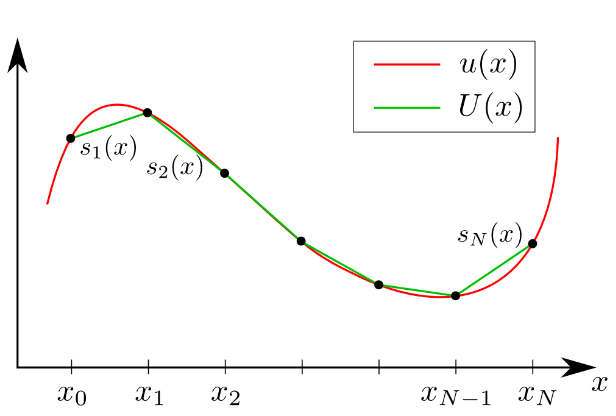
\includegraphics[width=0.5\linewidth]{spline.png}
  \caption{https://mipt.ru/upload/medialibrary/48a/splines.pdf}
\end{figure}

\medskip\noindent
Зададим функцию сплайна:
\begin{align*}
  U(x) = s_i(x), \; x \in [x_{i - 1}, x_i] \;\;
  s'_i(x) = s'_{i + 1}(x), \; s''_i(x) = s''_{i + 1}(x)
.\end{align*}
\[
s_i(x) = a_i + b_i (x - x_i) + \frac{c_i}{2} (x - x_i)^2 + \frac{d_i}{6} (x - x_i)^3
.\] 
\noindent
По аналогии с рядом Тейлора: \[
  a_i = s_i(x_i), \; b_i = s'_i(x_i), \; c_i = s''_i(x_i), \; d_i = s'''_i(x_i)
.\] 

\noindent
Пусть $h_i = (x_i - x_{i - 1})$.
Также введем ограничения на условия вторых производных на граничных точках: \[
  c_0 = 0, \; c_n = 0
.\] 
Таким образом, условия для интерполянты: 
\begin{align*}
& a_{i - 1} = a_i - b_i h_i + \frac{c_i}{2} h_i^2 - \frac{d_i}{6} h_i^3, & i =
  2,\dots,N& &(1) \\
& b_{i - 1} = b_i - c_i h_i + \frac{d_i}{2} h_i^2,  & i = 2,\dots,N & & (2) \\
& c_{i - 1} = c_i - b_i h_i,  & i=2,\dots,N & &(3)\\
& a_i = u(x_i), & i = 1,\dots,N & &(4) \\ 
& a_1 - b_1 h_1 + \frac{c_1}{2} h_i^2 - \frac{d_1}{6} h_i^3 = u(x_0)&\;& &(5)
\end{align*}

\noindent
Даляя произодя преобразования данных линейных уравнений получим матрицу вида: \[
A \cdot X = B
.\], где \[
A = 
\begin{pmatrix}
  2 & \frac{h_2}{h_1 + h_2} & \cdots \\
  \cdots & \cdots & \cdots\\
  \frac{h_i}{h_i + h_{i + 1}} & 2 & \frac{h_{i + 1}}{h_{i} + h_{i + 1}} \\
  \cdots & \cdots & \cdots \\
  \cdots & \frac{h_{N - 1}}{h_{N - 1} + h_{N}} & 2
\end{pmatrix}, \;\;
X = 
\begin{pmatrix}
c_1 \\
\vdots \\
c_i \\
\vdots \\
c_{N - 1}
\end{pmatrix},
B = 
\begin{pmatrix}
6 u(x_0, x_1, x_2) \\
\vdots \\
6 u(x_{i - 2}, x_{i - 1}, x_{i}) \\
\vdots \\
6 u(x_{N - 2}, x_{N - 1}, x_{N})
\end{pmatrix}
\]
Где: \[
   u(x_{i - 1}, x_{i}) = \frac{u(x_i) - u(x_{i - 1})}{x_i - x_{i - 1}} = \frac{a_i - a_{i -
   1}}{h_i}, \;\;
  u(x_{i - 2}, x_{i - 1}, x_i) = \frac{u_{x_{i - 1}, x_i} - u(x_{i - 2}, x_{i - 1})}{x_i - x_{i - 2}}
\] 

\noindent
Разрешив систему, получим требуемое.

\section{Блок схема численного метода.}

  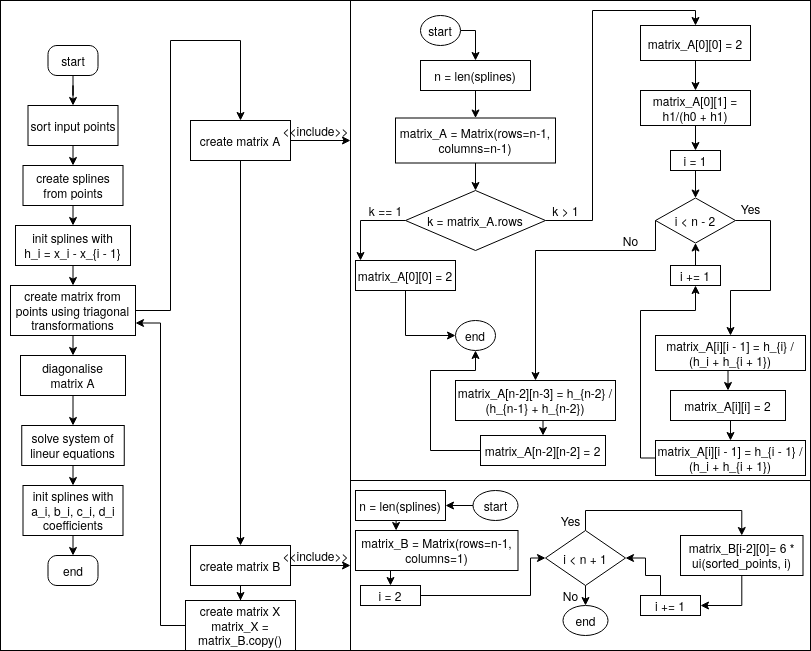
\includegraphics[width=\linewidth]{draw.png}


\bigskip
\section{Листинг реализованного численного метода.}

\begin{Verbatim}[fontsize=\small]
# функция для создания матрицы A

def create_with_triagonal_transformations(points, splines):
    matrix_a = _create_matrix_a(splines)
    matrix_b = _create_matrix_b(points)
    matrix_x = Matrix().init(matrix_b)
    return (matrix_a, matrix_b, matrix_x)


def fill_triagonal_transformed_splines(matrix_x, splines, sorted_points):
    c_arr = [0]
    for i in range(matrix_x.rows):
        c_arr.append(matrix_x[i][0])
    c_arr.append(0)
    for i in range(len(splines)):
        splines[i].a = _get_ai(sorted_points, i + 1)
        splines[i].b = _get_bi(sorted_points, i + 1, c_arr)
        splines[i].c = c_arr[i + 1]
        splines[i].d = _get_di(sorted_points, i + 1, c_arr)
    return


def _create_matrix_a(splines: list):
    n = len(splines)
    matrix_a = Matrix(rows=n - 1, columns=n - 1)
    if (matrix_a.rows > 1):
        matrix_a[0][0], matrix_a[0][1] = 2, (splines[1].get_hi() / (splines[0].get_hi() + 
          splines[1].get_hi()))
        for i in range(1, n - 2):
            matrix_a[i][i - 1] = splines[i].get_hi() / (splines[i].get_hi() + 
              splines[i + 1].get_hi())
            matrix_a[i][i] = 2
            matrix_a[i][i + 1] = splines[i + 1].get_hi() / (splines[i].get_hi() + 
              splines[i + 1].get_hi())
        matrix_a[n - 2][n - 3] = splines[n - 2].get_hi() / (splines[n - 1].get_hi() + 
          splines[n - 2].get_hi())
        matrix_a[n - 2][n - 2] = 2
    elif (matrix_a.rows == 1):
        matrix_a[0][0] = 2
    return matrix_a

def _create_matrix_b(sorted_points: list):
    n = len(sorted_points) - 1
    matrix_b = Matrix(rows=n-1, columns=1)
    for i in range(2, n + 1):
        matrix_b[i - 2][0] = 6 * _ui3(sorted_points, i)
    return matrix_b


def _ui2(sorted_points, index):
    p = sorted_points
    return (p[index]["y"] - p[index - 1]["y"]) / (p[index]["x"] - p[index - 1]["x"])

def _ui3(sorted_points, index):
    p = sorted_points
    return (_ui2(p, index) - _ui2(p, index - 1)) / (p[index]["x"] - p[index - 2]["x"])


def _get_ai(sorted_points: list, index: int):
    return sorted_points[index]["y"]

def _get_bi(sorted_points, index, c_arr):
    hi = sorted_points[index]["x"] - sorted_points[index - 1]["x"]
    ui = _ui2(sorted_points, index)
    return c_arr[index] * hi / 3 + c_arr[index - 1] / 6 * hi + ui

def _get_di(sorted_points, index, c_arr):
    hi = sorted_points[index]["x"] - sorted_points[index - 1]["x"]
    return (c_arr[index] - c_arr[index - 1]) / hi


# нахождение коэффициентов сплайнов 

class MultiSpline:
    def __init__(self, splines):
        self.splines = sorted(splines, key=lambda sp: sp.c_point_0)

    def calculate(self, x):
        i = 0
        while (i < len(self.splines) and x >= self.splines[i].c_point_0):
            i += 1
        if (i >= len(self.splines)):
            i -= 1
            if (self.splines[i].c_point_1 >= x):
                return self.splines[i].calculate(x)
            else:
                return None
        else:
            if (i == 0):
                if (self.splines[i].c_point_0 <= x):
                    return self.splines[i].calculate(x)
                else:
                    return None
            else:
                i -= 1
                return self.splines[i].calculate(x)

# END << class MultiSpline


class Spline:
    def __init__(self, c_point_0, c_point_1):
        self.c_point_0 = c_point_0
        self.c_point_1 = c_point_1
        self.a, self.b, self.c, self.d = None, None, None, None

    def calculate(self, x):
        if (self.a is None or self.b is None or self.c is None or self.d is None):
            raise ValueError("Uninitialized Spline")
        if not (self.c_point_0 <= x <= self.c_point_1):
            raise ValueError("x is out of range [%d %d]" % self.c_point_0 % self.c_point_1)

        return self.a + self.b * (x - self.c_point_1) + \
           self.c / 2 * (x - self.c_point_1) ** 2 + self.d / 6 * (x - self.c_point_1) ** 3

    def get_hi(self):
        return self.c_point_1 - self.c_point_0

    def __str__(self):
        return f"(a: {self.a}, b: {self.b}, c: {self.c}, d: {self.d}, " \
               f"c_point_0: {self.c_point_0}, c_point_1: {self.c_point_1})"

# END << class Spline


def get_splines(points):
    points = sorted(points, key=lambda p: p["x"])
    splines = []
    # initializing splines with hi
    for i in range(len(points) - 1):
        hi = Spline(points[i]["x"], points[i + 1]["x"])
        if (hi.get_hi() == 0):
            raise ProjectException("has points with same x coordinates")
        splines.append(hi)
    # creating matrices
    # matrix_a, matrix_b, matrix_x = create_with_simple_transformations(points, splines)
    matrix_a, matrix_b, matrix_x = create_with_triagonal_transformations(points, splines)
    # diagonalizing matrix, checking condition and solving
    if (not matrix_a.is_convergent()):
        raise ProjectException("matrix_a is not convergent")
    matrix_a = matrix_a.create_diagonal_max_if_can(matrix_b, matrix_x)[0]
    matrix_x = solve_iterate(matrix_a, matrix_b, matrix_x, diff=0.001)[0]
    # filling splines
    # fill_simple_transformed_splines(matrix_x, splines)
    fill_triagonal_transformed_splines(matrix_x, splines, points)
    return splines
\end{Verbatim}

\section{Примеры и результаты работы программы на разных данных.}

\noindentВвод данный через ifile:

\begin{verbatim}
data/task-4/input.json
{
    "equation": "\\sin x",
    "points": [
        {
            "x": 0.0,
            "y": 0.042887442205806564
        },
        {
            "x": 0.6,
            "y": 0.6563220848144425
        },
        {
            "x": 1.2,
            "y": 0.9687962468442449
        },
        {
            "x": 1.7999999999999998,
            "y": 1.0570729117576063
        },
        {
            "x": 2.4,
            "y": 0.7183530911521722
        },
        {
            "x": 3.0,
            "y": 0.07858772310639955
        }
    ]
}
\end{verbatim}


\begin{figure}[h]
  \centering
  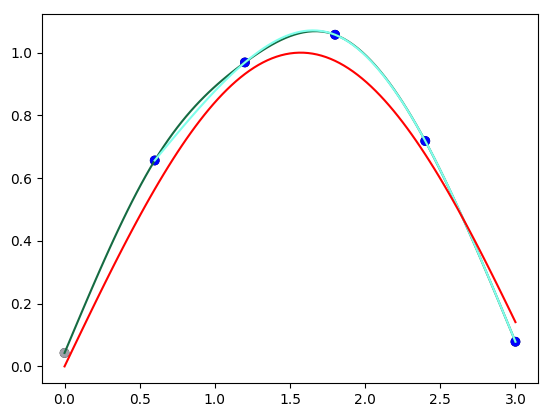
\includegraphics[width=0.5\textwidth]{sinux.png}
  \label{fig:sinux-png}
\end{figure}


\section{Вывод.}

В данной лабораторной работе был использован метод кубических сплайнов для вычисления значений
функции в промежуточных точках. Сложность данного алгоритма сопоставима с O(n) при использовании 
метода прогонки для вычисления СЛАУ, а у метода Ньютона и Лагранжа сложность O($n^2$).
 
\medskip\noindent
Ошибка функции стремится к 0 при увеличении количества узлов интерполяции. В отличие от методов
Лагранжа и Ньютона, где используются многочлены, погрешность данного метода будет выше при
сопоставимом количестве узлов интерполяции, так как их погрешность оценивается остаточным членом,
а у метода кубических сплайнов используются многочлены 3 степени.

\medskip\noindent
Для нахождения точки с наибольшей погрешностью оценивалось ее отклонение по оси y. После ее
нахождения эта точка удаляется, и сплайны перестраиваются.

\bigskip\noindent
В ходе выполнения лабораторной работы узнал об этих трех методах интерполяции, о методе прогонки и
трехдиагольной матрице.

\end{document}

